\documentclass{article}

\usepackage{graphicx}
\usepackage{hyperref}
\usepackage[a4paper, margin=1.25in]{geometry}
\usepackage{breakcites}
\usepackage{subcaption}
\usepackage{float}
\usepackage{textcomp}
\usepackage{amsmath}
\usepackage{textgreek}
\usepackage{authblk}
\usepackage{rotating}
\usepackage{booktabs}
\usepackage{longtable}
\usepackage{pdflscape}
\usepackage{subcaption}
\usepackage{lineno}
\usepackage{fancyhdr}
\usepackage[
  style=numeric,
  citestyle=numeric-comp,
  backend=biber,
  doi=true,
  natbib=true,
  sorting=none
]{biblatex}

\pagestyle{fancy}
\fancyhf{}
\lfoot{Supplemental Materials for \textit{Fine-scale Twitter Big Data Reveals Neighborhood Inequalities in Mental Health Effects of High Temperatures}}
\rfoot{\thepage}

\renewcommand{\footrulewidth}{0.4pt}
\renewcommand{\headrulewidth}{0pt}


\addbibresource{TextDataClimateShocks.bib}

\begin{document}
\begin{center}
\section*{Supplemental Materials for \textit{Fine-scale Twitter Big Data Reveals Neighborhood Inequalities in Mental Health Effects of High Temperatures}}
\end{center}

%Supplement will have:

%Equations used for RH and WBGT

\section{Alternative Parameterizations}

\section{Effects of Precipitation and Sunshine}

\section{Alternative Sentiment Algorithm}

\setcounter{table}{0}
\setcounter{figure}{0}
\setcounter{section}{0}
\renewcommand{\thetable}{S\arabic{table}}
\renewcommand{\thefigure}{S\arabic{figure}}
\renewcommand{\thesection}{S\arabic{section}}

\section*{Supplemental Info}
\setcounter{table}{0}
\setcounter{figure}{0}
\setcounter{section}{0}
\renewcommand{\thetable}{S\arabic{table}}
\renewcommand{\thefigure}{S\arabic{figure}}
\renewcommand{\thesection}{S\arabic{section}}

\begin{figure}[H]
  \centering
  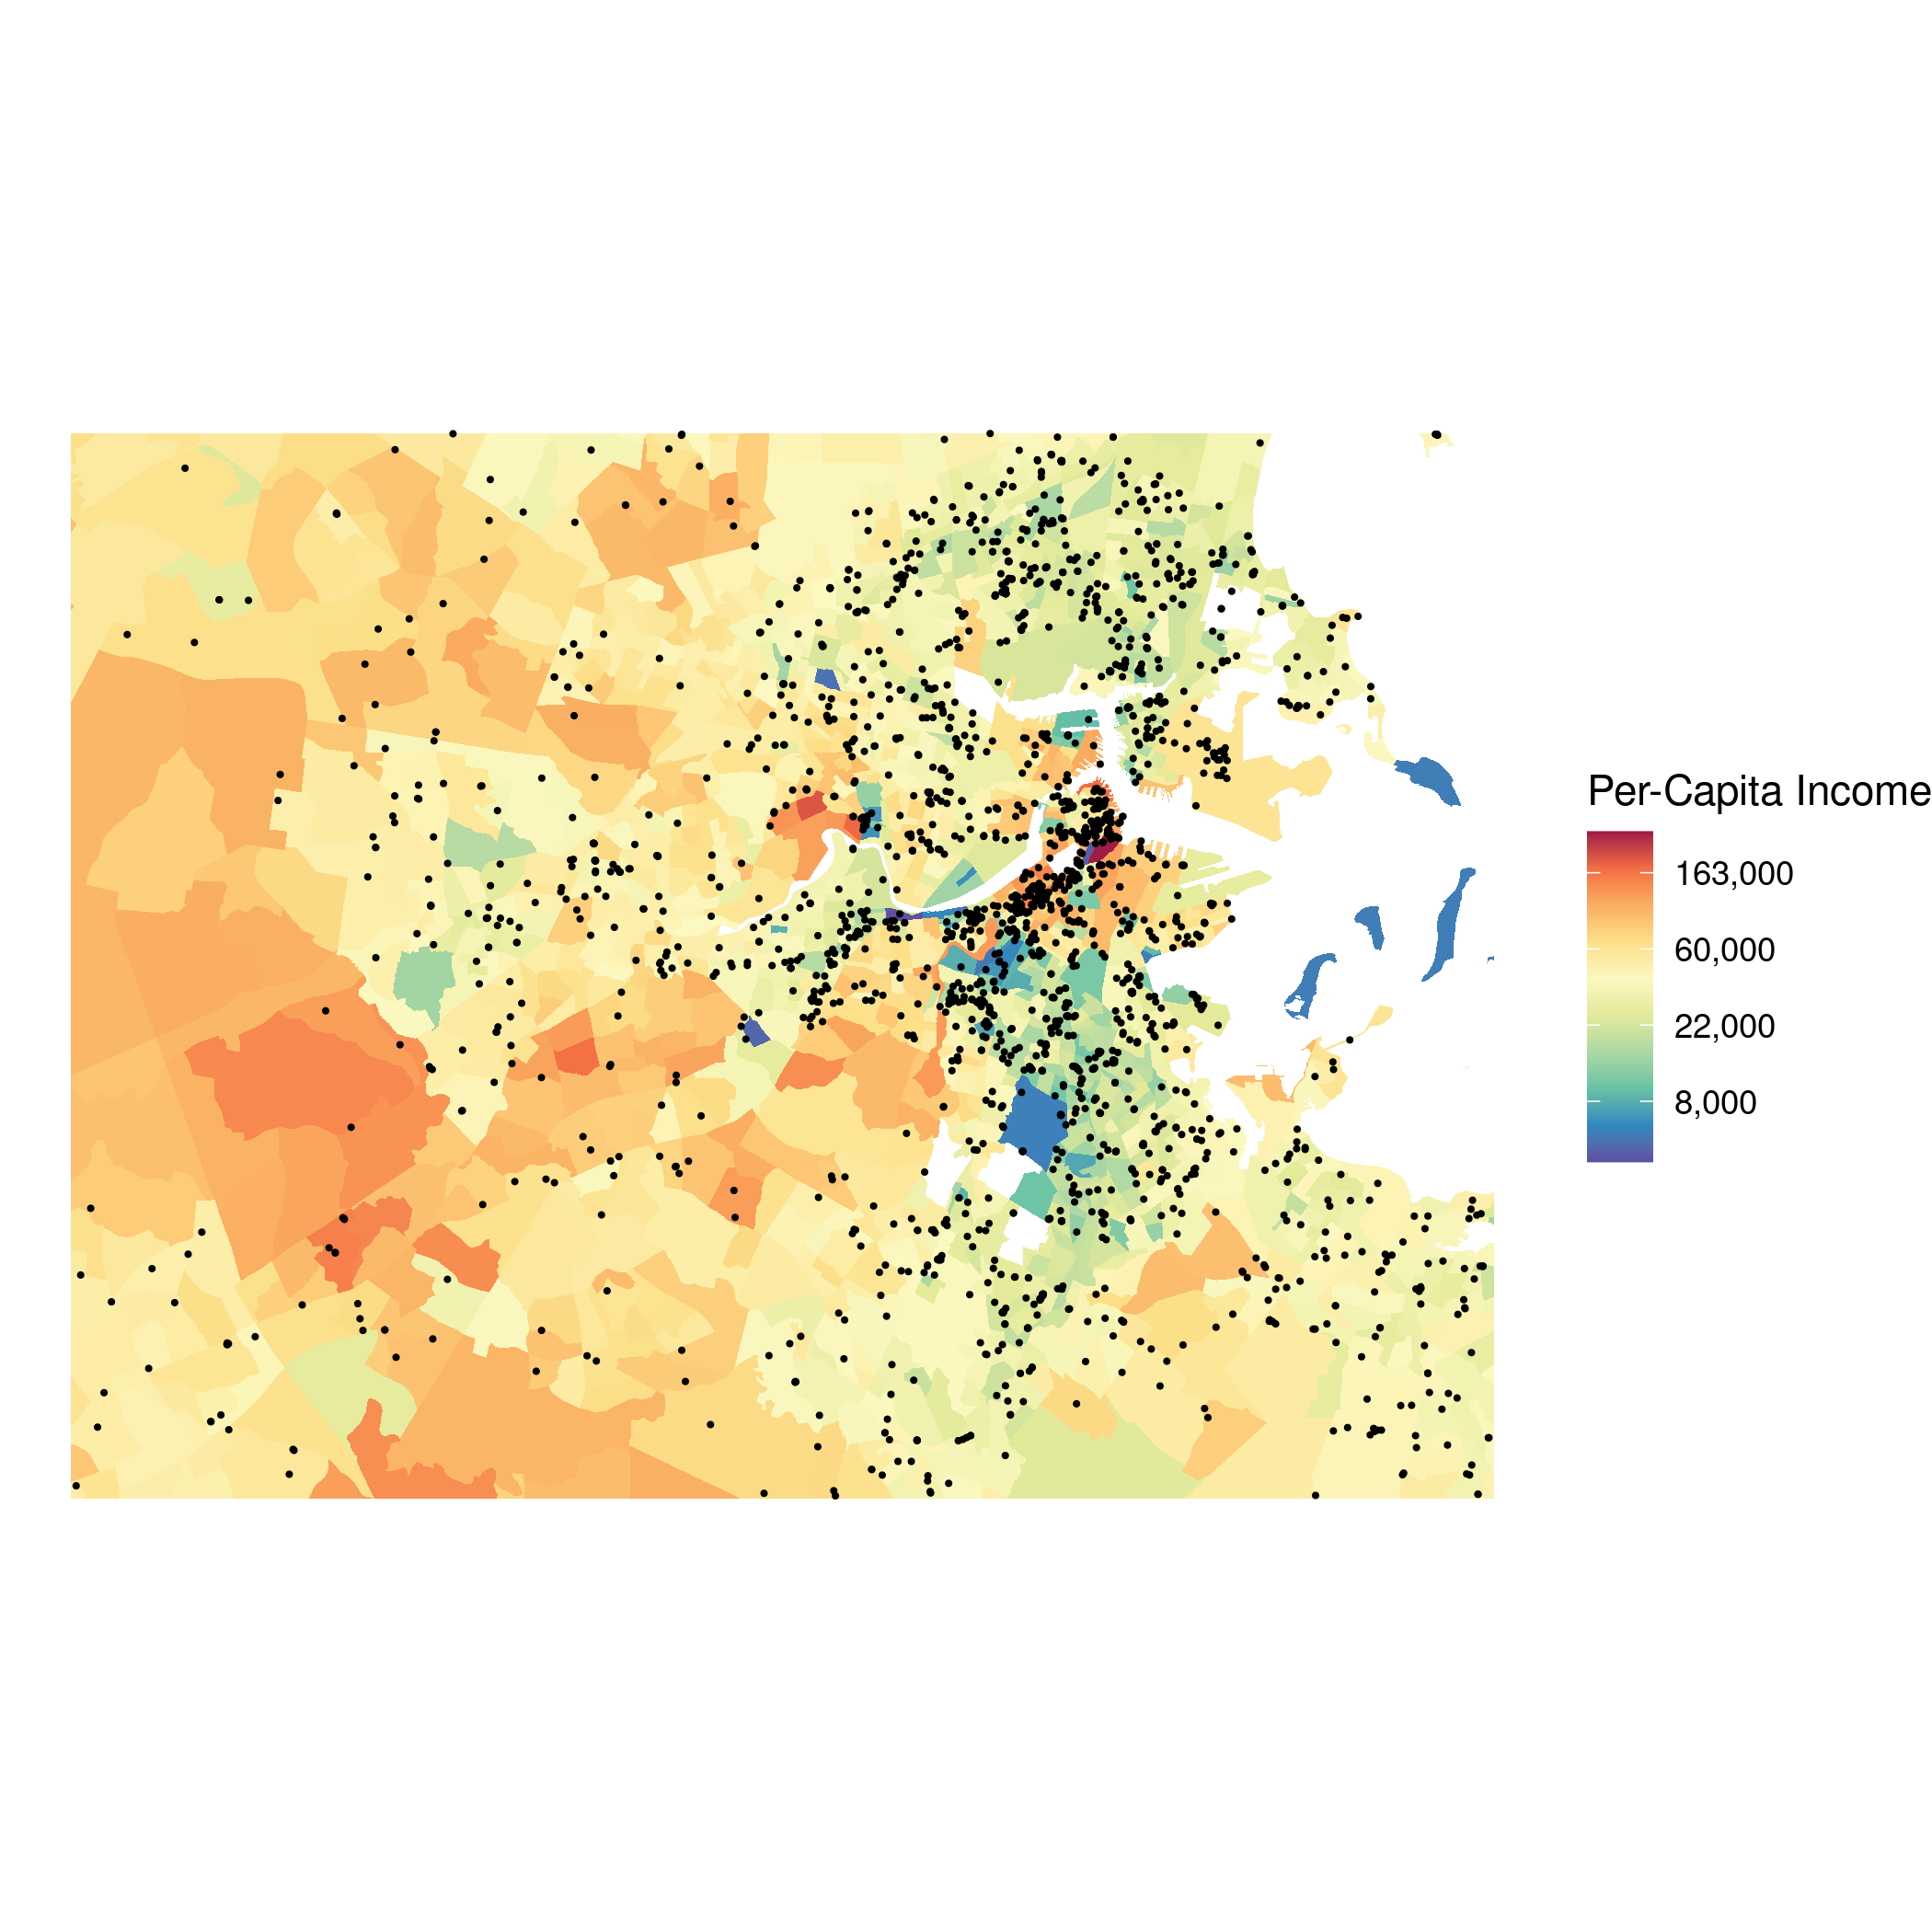
\includegraphics[width=\linewidth]{../res/Boston_Map.png}
  \caption{Here is a map of all tweets in boston, overlaid with income by census block}
  \label{fig:timeseries}
\end{figure}

\begin{figure}[H]
  \centering
  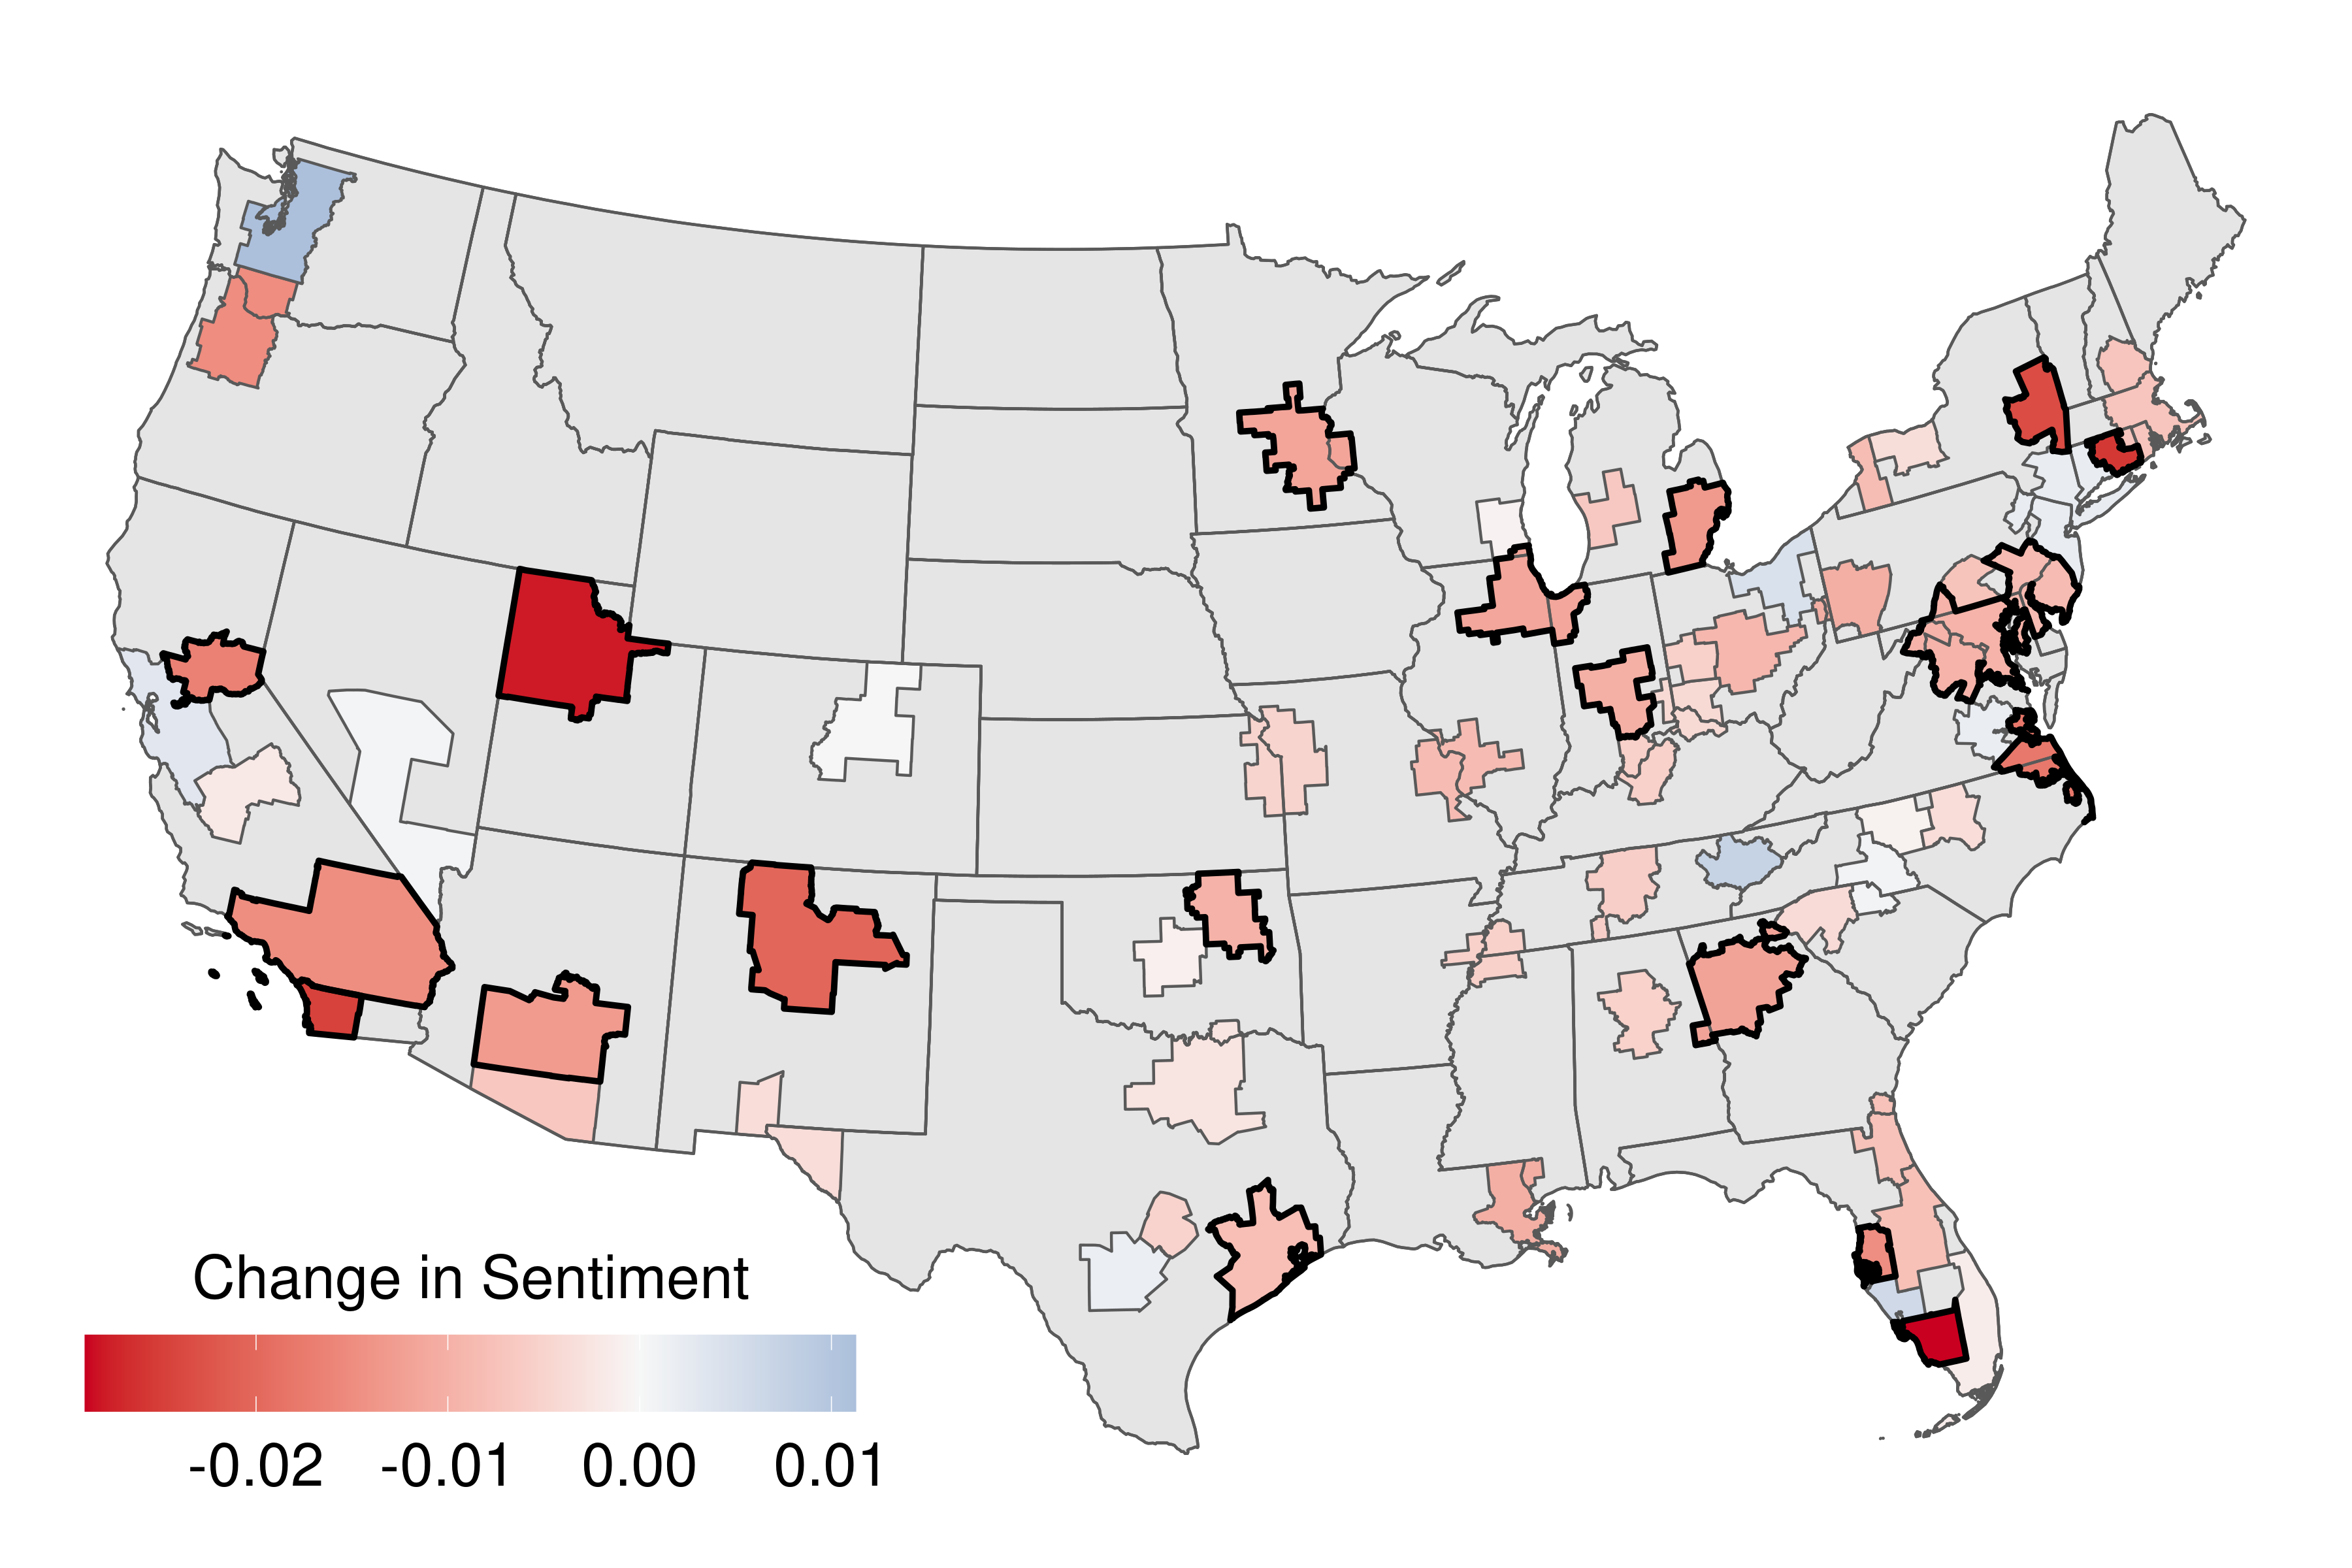
\includegraphics[width=\linewidth]{../res/map_wbgt.png}
  \caption{Here is a map of all tweets in boston, overlaid with income by census block}
  \label{fig:timeseries}
\end{figure}

% Show results with hedonometer and AFINN

% Show results with income binned and race continuous

% Entire analysis by income-race together



\subsection{Effects by Time of Day}

In addition to providing data with high spatial resolution, twitter data also comes with very high temporal resolution as each tweet is time-stamped.  Thus, we were able to examine the impact of heat on sentiment for each hour of the day (See Fig. \ref{fig:ts-wbgt}).  We found that heat decreased expressed sentiment at nearly all hours of the day, and that heat had the largest effect on sentiment early in the morning, between 4am and 6am.  Heat had the weakest effects on sentiment at midday, and at 3am.

\begin{figure}[H]
  \centering
  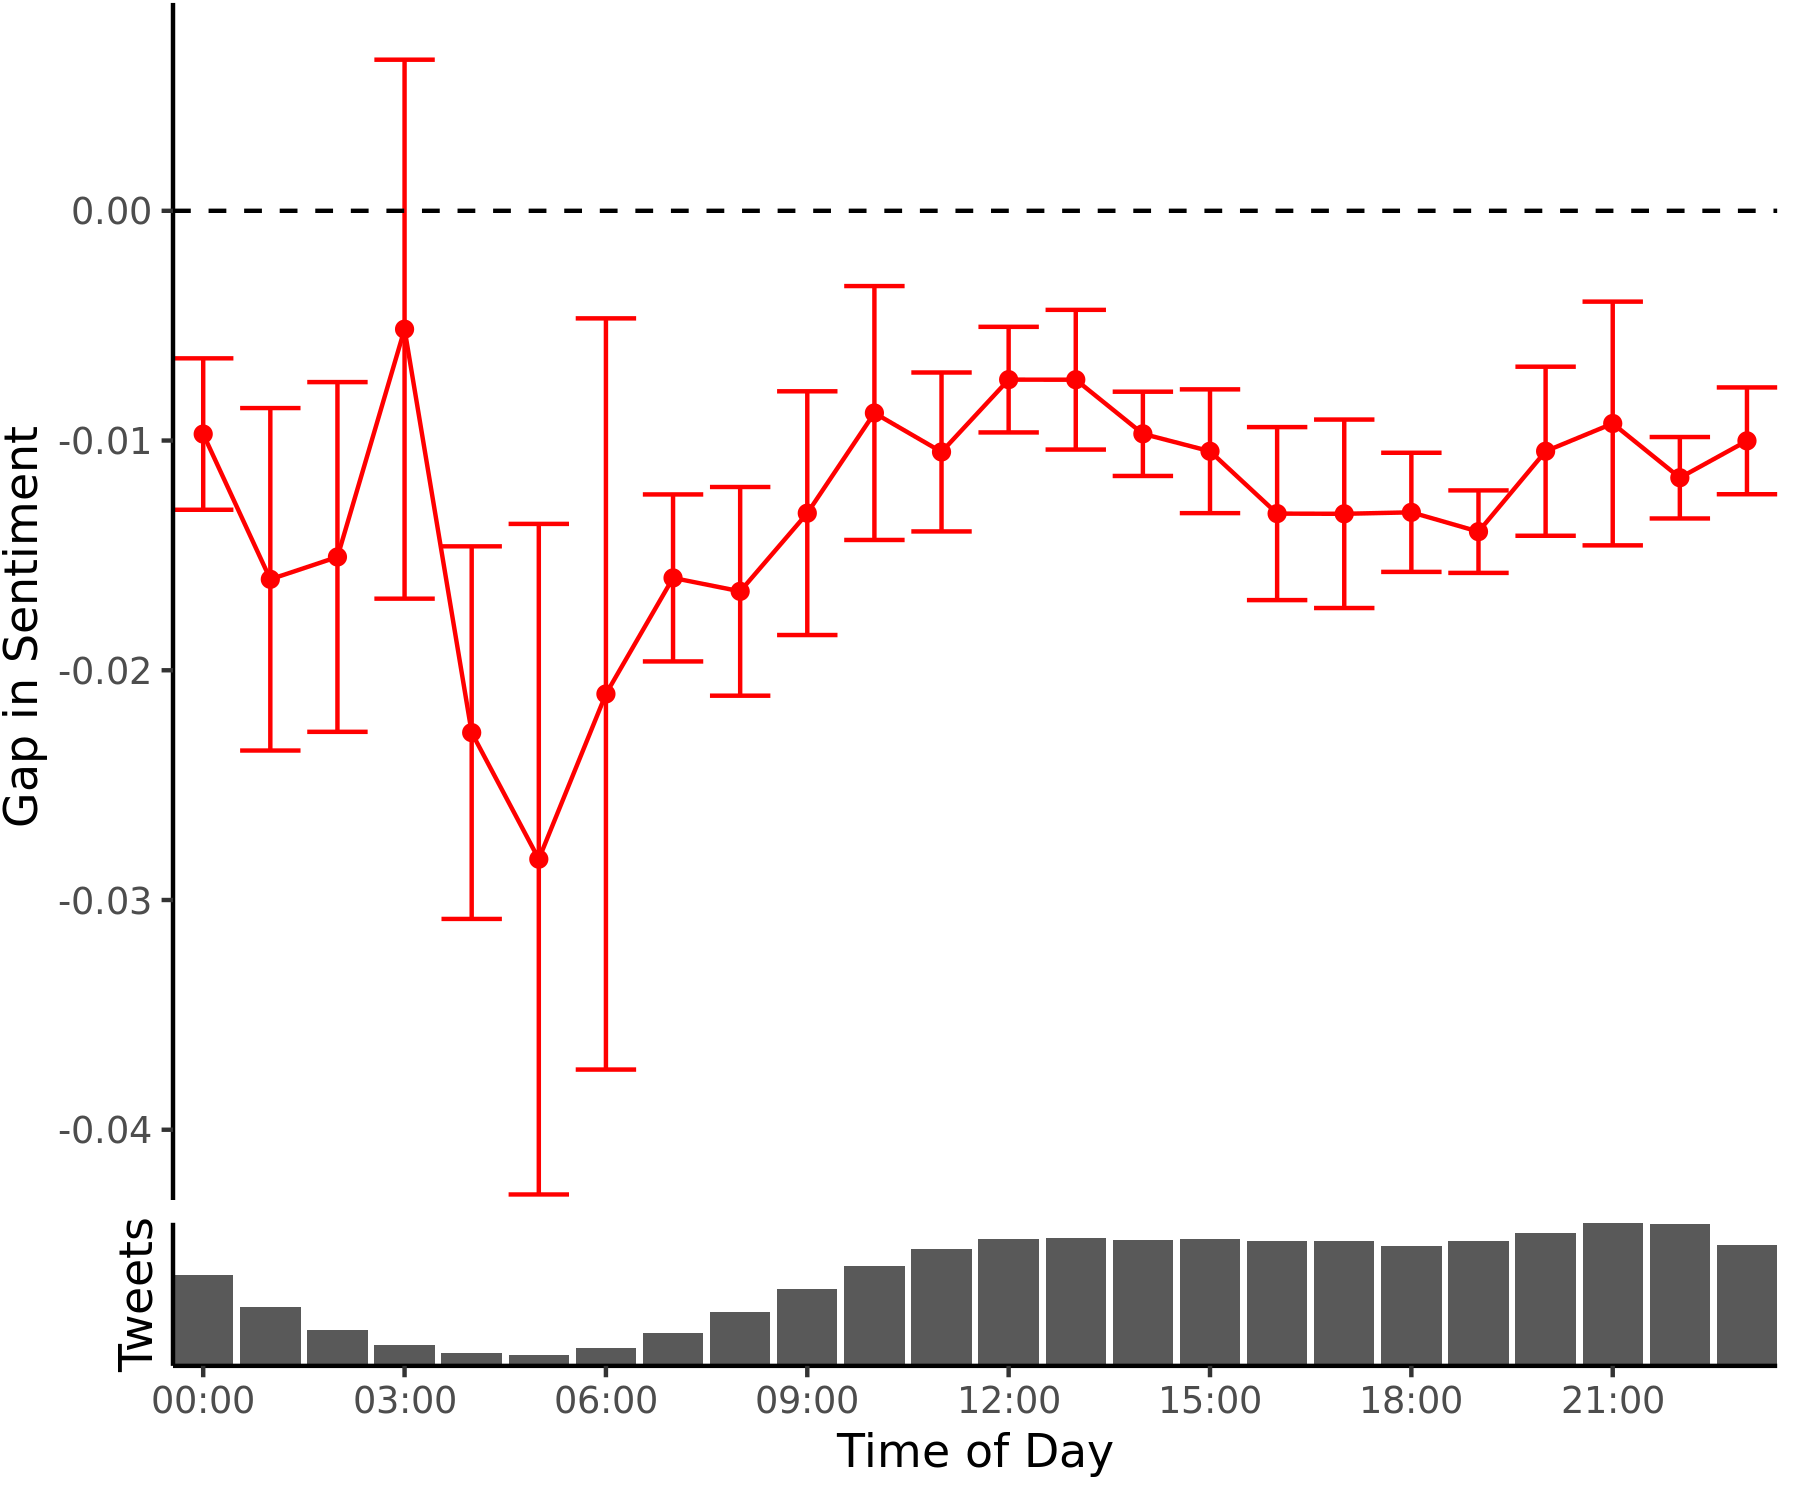
\includegraphics[width=0.5\linewidth]{../res/ts.png}
  \caption{Effects of rising temperatures on sentiment by hour of the day, with a 95\% confidence interval.  The value shown is the predicted change in VADER score for a 25-degree increase in temperatures.}
  \label{fig:ts-wbgt}
\end{figure}

% Interpret Time Series Analysis
Recent research has suggested that the impacts of heat on sleep quality may play a large role in the observed mental health effects of heat \cite{Obradovich2017May, Mullins2019Dec}, and our temporal analysis was able to examine this hypothesis.  While our estimates were more uncertain at night due to a lower volume of tweets, we found much stronger effects of heat on expressed sentiment in the early morning, adding weight to the sleep quality pathway linking heat and mental health that other authors have found.  This suggests that efforts to improve mental health during heat waves may have the largest impact by focusing on providing electricity and air conditioning at night.


\subsubsection{Hedonometer}
The Hedonometer \cite{dodds_temporal_2011} is a corpus-based technique to get sentiment score from multi-lingual texts. The core steps are (1) building human evaluations of the happiness of a set of individual words, and (2)using a naive algorithm for scaling up from individual words to texts. For the English corpus, Dodds and others \cite{dodds_temporal_2011} collect 10,222 unique words and used crowd-sourcing platform Amazon Mechanical Turk to get human evaluation of happiness degree for each word in an integer scale from 1 to 9, representing a sad to happy spectrum. Score 5 represents neutral words. Each word will be calculated average score and then the word and happiness score are compiled into a dataset (labMT 1.0). Some illustrative example of words are: 

\[h_{avg} (\text{laughter}) = 8.50 \]
\[h_{avg} (\text{the}) = 4.98\]
\[h_{avg} (\text{hate}) = 2.34\]

The sentiment score for single text will be the mean happiness score for all words in the text.


\printbibliography

\end{document}
